% --------------------------------------------------------------
% This is all preamble stuff that you don't have to worry about.
% Head down to where it says "Start here"
% --------------------------------------------------------------
 
\documentclass[12pt]{article}
 
\usepackage[margin=1in]{geometry} 
\usepackage{amsmath,amsthm,amssymb}
\usepackage{graphicx} 
\graphicspath{ {./images/} }
 
\newcommand{\N}{\mathbb{N}}
\newcommand{\Z}{\mathbb{Z}}
\newcommand\gldec[2]{
\underset{#1}{\overset{#2}{\gtrless}}
}
 
\newenvironment{theorem}[2][Theorem]{\begin{trivlist}
\item[\hskip \labelsep {\bfseries #1}\hskip \labelsep {\bfseries #2.}]}{\end{trivlist}}
\newenvironment{lemma}[2][Lemma]{\begin{trivlist}
\item[\hskip \labelsep {\bfseries #1}\hskip \labelsep {\bfseries #2.}]}{\end{trivlist}}
\newenvironment{exercise}[2][Exercise]{\begin{trivlist}
\item[\hskip \labelsep {\bfseries #1}\hskip \labelsep {\bfseries #2.}]}{\end{trivlist}}
\newenvironment{reflection}[2][Reflection]{\begin{trivlist}
\item[\hskip \labelsep {\bfseries #1}\hskip \labelsep {\bfseries #2.}]}{\end{trivlist}}
\newenvironment{proposition}[2][Proposition]{\begin{trivlist}
\item[\hskip \labelsep {\bfseries #1}\hskip \labelsep {\bfseries #2.}]}{\end{trivlist}}
\newenvironment{corollary}[2][Corollary]{\begin{trivlist}
\item[\hskip \labelsep {\bfseries #1}\hskip \labelsep {\bfseries #2.}]}{\end{trivlist}}
 
\begin{document}
 
% --------------------------------------------------------------
%                         Start here
% --------------------------------------------------------------
 
%\renewcommand{\qedsymbol}{\filledbox}
 
\title{Homework Assignment # 4}
\author{Rushabh Ashok Dharia\\ 
CSCI-B555 Machine Learning} 
\maketitle
\begin{multline*}
    \text{\textbf{Note: }Homework was discussed with Varun Miranda}
\end{multline*} 
\begin{theorem}[Ans]{1}
\text{Explanation}\\
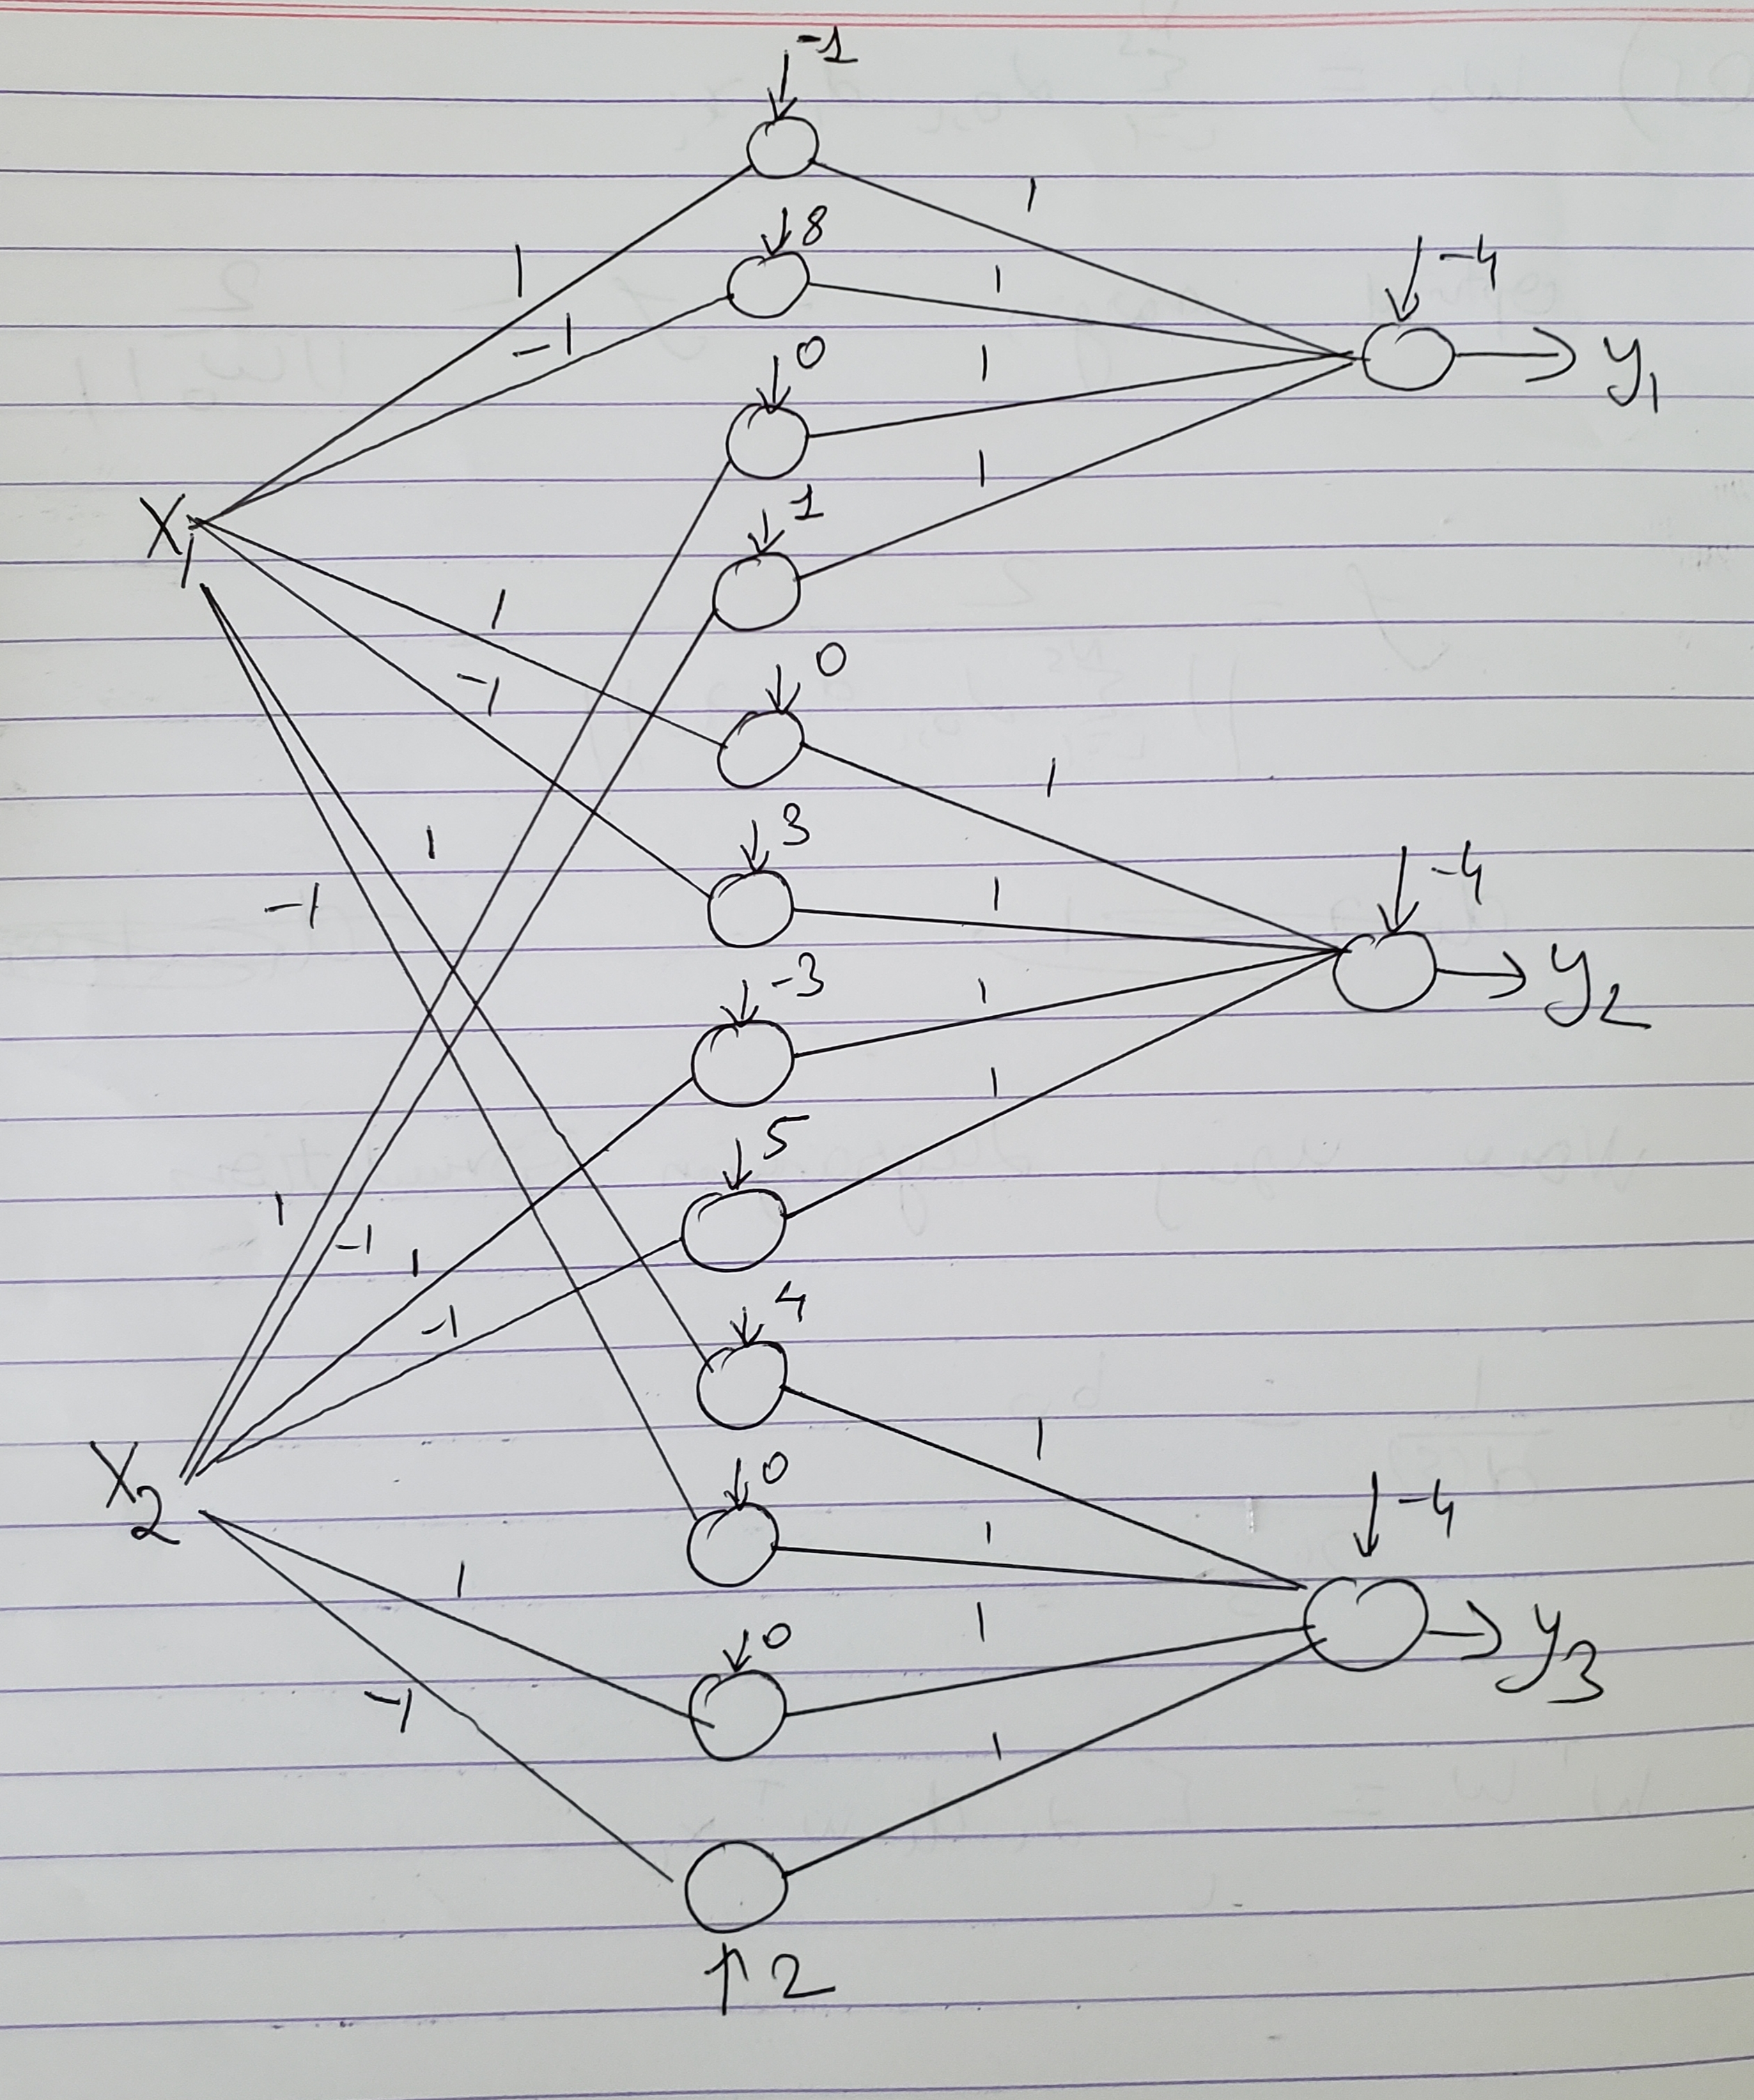
\includegraphics[scale=0.1]{q1}\\
\text{As mentioned in the question we need to design a Neural Network with 3 output units}\\
\text{we can consider that Class 4 is recognized when $y_{i}$ = -1 for } 1 \leq i \leq 3 \\
\text{This means that when all neurons in the last layer do not fire (or output -1) we can}\\
\text{say that the point belongs to class 4. This can be easily showed by adding another}\\
\text{layer which will take the outputs $y_{1}$, $y_{2}$ and $y_{3}$ as inputs} \\ \\
\text{Consider the first 4 neurons in the 1st Layer}\\
\text{1st Neuron will output 1 if } x_{1} \geq 1 \text{, otherwise 0}\\ 
\text{2nd Neuron will output 1 if } x_{1} \leq 8 \text{, otherwise 0}\\
\text{3rd Neuron will output 1 if } x_{2} \geq 0 \text{, otherwise 0}\\ 
\text{4th Neuron will output 1 if } x_{2} \leq 1 \text{, otherwise 0}\\ 
\text{Now, the 1st Neuron in the 2nd Layer will output 1 if all 4 neurons mentioned above output 1,} \\
\text{else it will output 0}\\
\text{Similarly, the other 2 classes can be determined}
\end{theorem}
\begin{theorem}[Ans]{2}
\begin{proof}[a)]
\begin{align*}
J(u_{j}) &= \sum_{j=1}^{K} \sum_{i=1}^{N} w_{ij} ||x_{i}-u_{j}||^{2}\\
&= \sum_{j=1}^{K} \sum_{i=1}^{N} w_{ij} (x_{i}^{2}+u_{j}^{2} - 2x_{i}u_{j})\\
&= \sum_{j=1}^{K} \sum_{i=1}^{N} w_{ij}x_{i}^{2}+w_{ij}u_{j}^{2} - 2w_{ij}x_{i}u_{j}\\
\text{Taking derivative w.r.t }& u_{j} \text{ and setting it equal to 0} \\
\frac{d J(u_{j})}{d u_{j}} &= \sum_{j=1}^{K} \sum_{i=1}^{N} 0 + 2w_{ij}u_{j} - 2w_{ij}x_{i} = 0\\
\sum_{j=1}^{K} \sum_{i=1}^{N}w_{ij} u{j} &=  \sum_{j=1}^{K} \sum_{i=1}^{N}w_{ij}x_{i}\\
\text{Therefore, } \hat{u_{j}} &= \frac{\sum_{i=1}^{N} w_{ij}x_{i}}{\sum_{i=1}^{N}w_{ij}}
\end{align*}
\end{proof}
\begin{proof}[b)]
\text{Numerator denotes the points in each cluster and the denominator denotes the}\\
\text{number of points in each cluster. The fraction as a whole denotes the weighted average}\\
\text{of all points in the cluster}\\
\begin{align*}
\end{align*}
\end{proof}
\end{theorem}
\begin{theorem}[Ans]{3}
\begin{proof}[a)]
\begin{align*}
    y(i) &= \sum_{j=1}^{K} w_{j}(n)e^{\frac{||x_{i} - u_{j}(n)||^{2}}{2\sigma^{2}(n)}}\\
    \frac{\partial y(i)}{\partial w_{j}(n)} &= \sum_{j=1}^{K}e^{\frac{||x_{i} - u_{j}(n)||^{2}}{2\sigma^{2}(n)}}\\
    \frac{\partial y(i)}{\partial u_{j}(n)} &= w_{j}(n)e^{\frac{||x_{i} - u_{j}(n)||^{2}}{2\sigma^{2}(n)}}.\frac{x_{i} - u_{j}(n)}{\sigma^{2}(n)}\\
    \frac{\partial y(i)}{\partial \sigma(n)} &= w_{j}(n)e^{\frac{||x_{i} - u_{j}(n)||^{2}}{2\sigma^{2}(n)}}.\frac{(x_{i} - u_{j}(n))^{2}}{\sigma^{3}(n)}\\
    \text{Now, } E &= \frac{1}{2}  \sum_{i=1}^{N}(d(i)-y(i))^{2}\\
    \frac{\partial E}{\partial w_{j}(n)} &= - \sum_{i=1}^{N}(d(i)-y(i)).\frac{\partial y(i)}{\partial w_{j}(n)}\\
    &= - \sum_{i=1}^{N}(d(i)-y(i))\sum_{j=1}^{K}e^{\frac{||x_{i} - u_{j}(n)||^{2}}{2\sigma^{2}(n)}}\\
    \frac{\partial E}{\partial u_{j}(n)} &= - \sum_{i=1}^{N}(d(i)-y(i)).\frac{\partial y(i)}{\partial u_{j}(n)}\\
    &= - \sum_{i=1}^{N}(d(i)-y(i))\sum_{j=1}^{K}w_{j}(n)e^{\frac{||x_{i} - u_{j}(n)||^{2}}{2\sigma^{2}(n)}}.\frac{x_{i} - u_{j}(n)}{\sigma^{2}(n)}\\
    \frac{\partial E}{\partial \sigma(n)} &= - \sum_{i=1}^{N}(d(i)-y(i)).\frac{\partial y(i)}{\partial \sigma(n)}\\
    &= - \sum_{i=1}^{N}(d(i)-y(i))\sum_{j=1}^{K}w_{j}(n)e^{\frac{||x_{i} - u_{j}(n)||^{2}}{2\sigma^{2}(n)}}.\frac{||x_{i} - u_{j}(n)||^{2}}{\sigma^{3}(n)}\\
\end{align*}
\end{proof}
\begin{proof}[b)]
\begin{align*}
    w_{kj}(n+1) &= w_{kj}(n) - \eta_{w}\frac{\partial E}{\partial w_{kj}}\\
    &= w_{kj}(n) + \eta_{w} \sum_{i=1}^{N}(d(i)-y(i))\sum_{j=1}^{K}e^{\frac{||x_{i} - u_{j}(n)||^{2}}{2\sigma^{2}(n)}}\\
    w_{kj}(n+1) &= w_{kj}(n) - \eta_{u}\frac{\partial E}{\partial u}\\
    &= w_{kj}(n) + \eta_{u}\sum_{i=1}^{N}(d(i)-y(i))\sum_{j=1}^{K}w_{j}(n)e^{\frac{||x_{i} - u_{j}(n)||^{2}}{2\sigma^{2}(n)}}.\frac{x_{i} - u_{j}(n)}{\sigma^{2}(n)}\\
    w_{kj}(n+1) &= w_{kj}(n) - \eta_{\sigma}\frac{\partial E}{\partial \sigma}\\
    &= w_{kj}(n) - \eta_{\sigma}\sum_{i=1}^{N}(d(i)-y(i))\sum_{j=1}^{K}w_{j}(n)e^{\frac{||x_{i} - u_{j}(n)||^{2}}{2\sigma^{2}(n)}}.\frac{||x_{i} - u_{j}(n)||^{2}}{\sigma^{3}(n)}\\
\end{align*}
\end{proof}
\end{theorem}
\begin{theorem}[Ans]{4}
\begin{proof}[a)]Plot\\
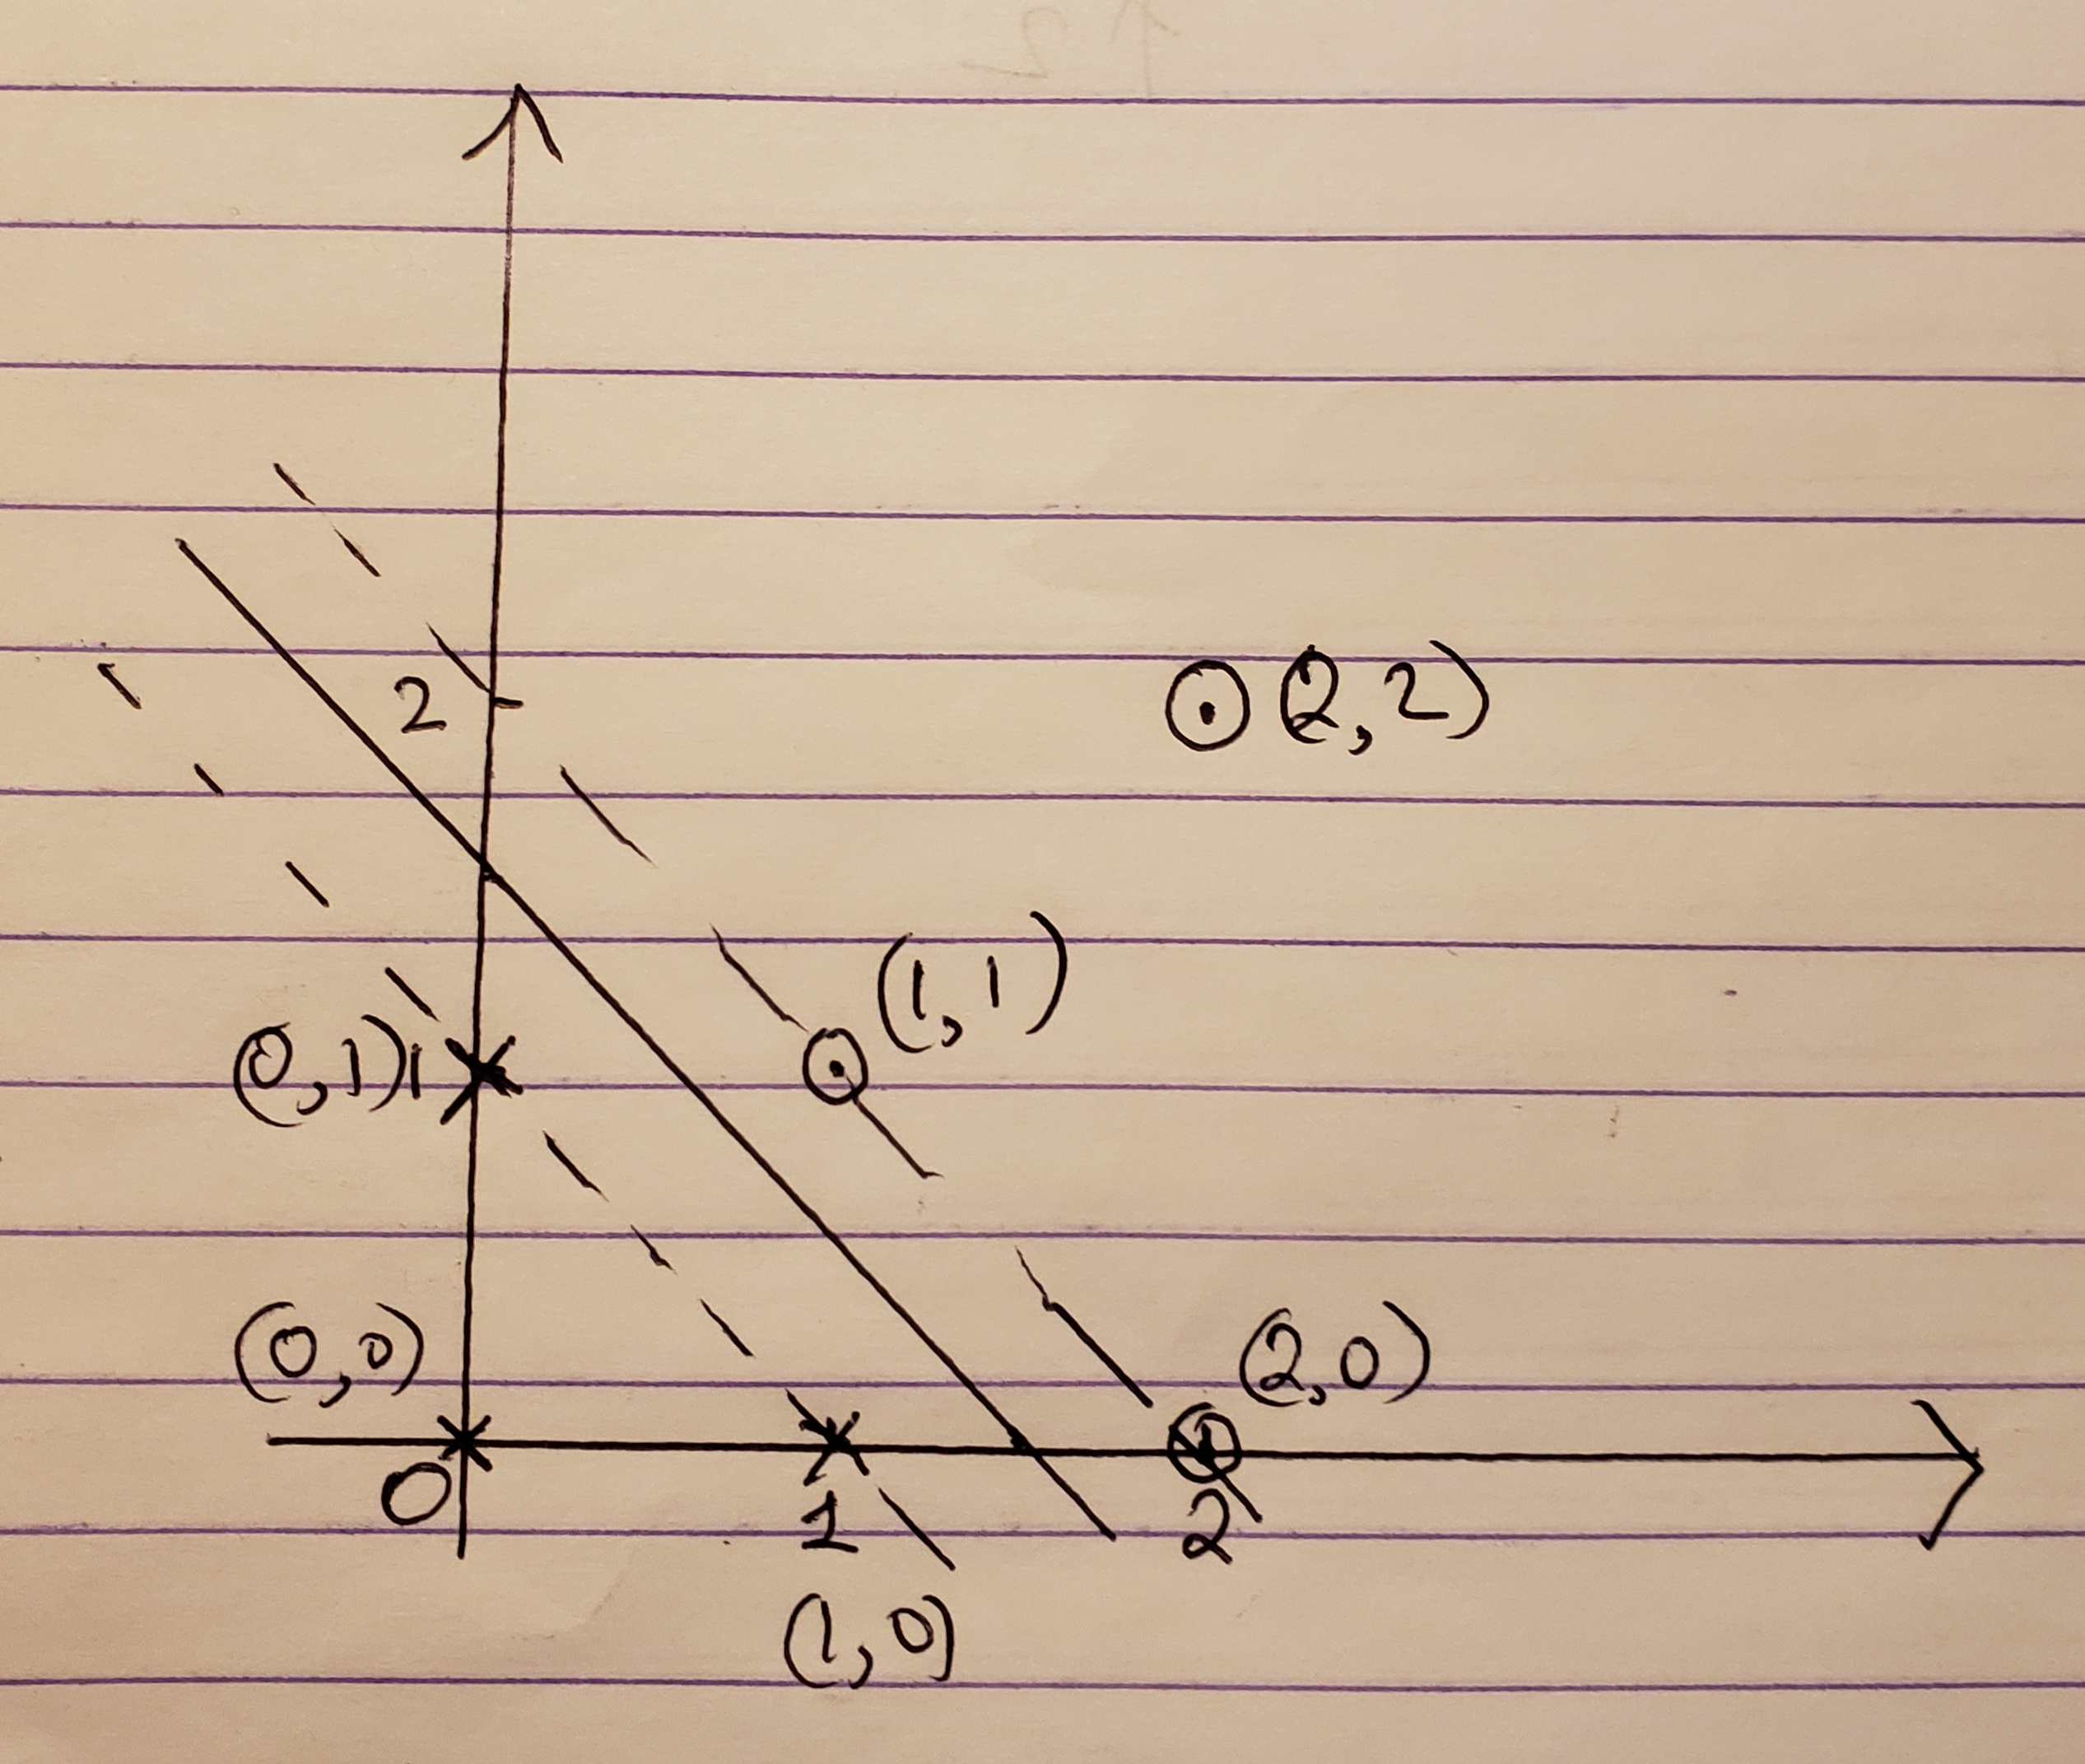
\includegraphics[scale=0.15]{q4}
\pagebreak
\begin{align*}
[w_{1} \hspace{2mm} w_{2}]^{T}[2 \hspace{2mm} 0] + b_{0} &= 1 \\
[w_{1} \hspace{2mm} w_{2}]^{T}[1 \hspace{2mm} 1] + b_{0} &= 1 \\
2w_{1} + b_{0} &= 1 \hspace{10mm} (1)\\
w_{1} + w_{2} + b_{0} &= 1 \hspace{10mm} (2)\\
\text{Subtracting (2) from (1)}\\
w_{1} - w_{2} &= 0\\
w_{1} &= w_{2}  \hspace{10mm} (3)\\
\\
[w_{1} \hspace{2mm} w_{2}]^{T}[1 \hspace{2mm} 0] + b_{0} &= -1 \\
w_{1}+b_{0}&=-1 \hspace{10mm} (4)\\
\text{Subtracting (1) from (4)}\\
-w_{1} &= -2\\
w_{1} &= 2  \hspace{10mm} (5)\\
w_{2}  &= 2  \hspace{10mm} \text{Using (3) and (5)}\\
b_{0} &= -3  \hspace{10mm} \text{Using (4) and (5)}\\
\end{align*}
\end{proof}
\begin{proof}[b)]
\begin{align*}
\text{The Support Vectors are (0,1), (1,0), (1,1) and (2,0}
\end{align*}
\end{proof}
\end{theorem}
\begin{theorem}[Ans]{5}
\begin{align*}
J(w,b,\alpha)  &= \frac{w^{T}w}{2} - \sum_{i}^{N}\alpha_{i}[d_{i} (w^{T}x+b)-1]\\
\phi(w) &= \frac{1}{2} w^{T}w\\
\text{Now, }\phi(w) &= J(w,b,\alpha)\\
\text{Therefore, }&\sum_{i}^{N}\alpha_{i}[d_{i} (w^{T}x+b_{0})-1] = 0\\
& \sum_{i}^{N}\alpha_{i}d_{i}w^{T}x+\sum_{i}^{N}\alpha_{i}d_{i}b_{0} - \sum_{i}^{N}\alpha_{i} = 0 \hspace{10mm} (1)\\
\text{Now, } &w = \sum_{i}^{N}\alpha_{i}d_{i}x\\
\text{Therefore, } &w^{T}w = \sum_{i}^{N}\alpha_{i}d_{i}w^{T}x \hspace{10mm} (2)\\
&\sum_{i}^{N}\alpha_{i}d_{i} = 0 \hspace{10mm} (3)\\
& \text{Substituting (2) and (3) in (1)}\\
 &w^{T}w + 0 - \sum_{i}^{N}\alpha_{i} = 0 \\
 &w^{T}w = \sum_{i}^{N}\alpha_{i}\\
 &||w|| = (\sum_{i}^{N}\alpha_{i})^{1/2} \hspace{10mm} (4)\\
 &\text{Now, }\rho = \frac{2}{||w||}\\
 \text{Therefore, }& \rho = \frac{2}{(\sum_{i}^{N}\alpha_{i})^{1/2}} \hspace{10mm} \hspace{10mm} \text{Using, }(4)
\end{align*}
\end{theorem}
\pagebreak

% --------------------------------------------------------------
%     You don't have to mess with anything below this line.
% --------------------------------------------------------------
 
\end{document}